\chapter{External Interface}
\label{appendix:external-interface}

\subsection{Chip Layout}

The SIRC CPU is most commonly provided as a DIP-64 package.

\begin{figure}[htbp]
	\centering
	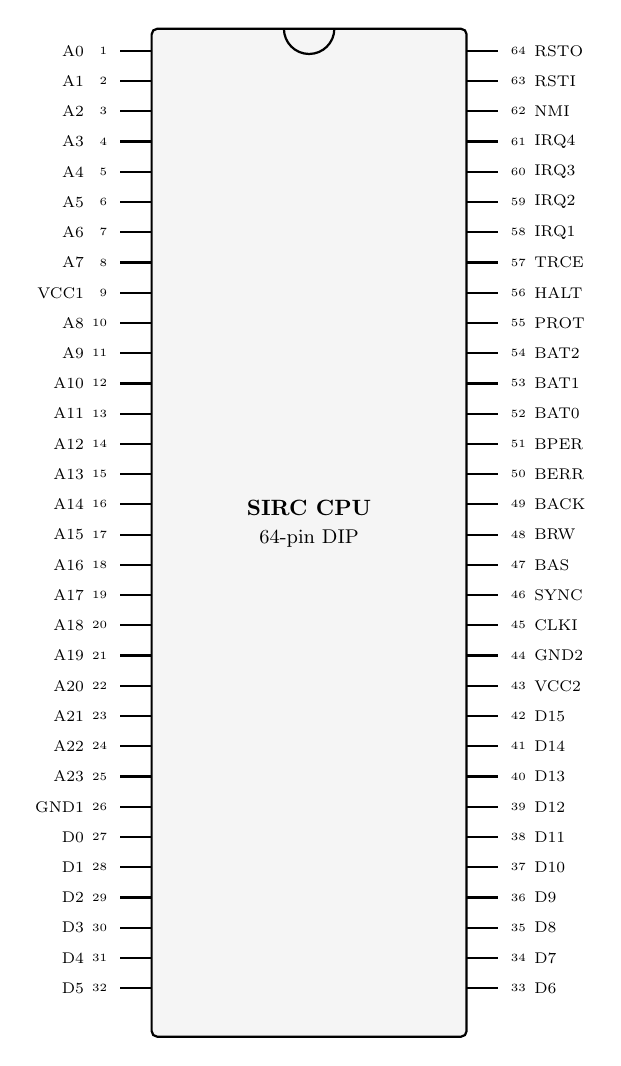
\begin{tikzpicture}[
			scale=0.8,
			transform shape,
			pinlabel/.style={font=\scriptsize},
			pinnum/.style={font=\tiny},
			body/.style={draw, thick, rounded corners=2pt, fill=gray!8},
			pin/.style={draw, thick}
		]

		% Package body
		\draw[body] (0,0) rectangle (5,-16);

		% Notch
		\draw[thick] (2.1,0) arc[start angle=180,end angle=360,radius=0.4];

		% Left-side pins: 1-32, top to bottom
		\foreach \n/\name in {
				1/A0,
				2/A1,
				3/A2,
				4/A3,
				5/A4,
				6/A5,
				7/A6,
				8/A7,
				9/VCC1,
				10/A8,
				11/A9,
				12/A10,
				13/A11,
				14/A12,
				15/A13,
				16/A14,
				17/A15,
				18/A16,
				19/A17,
				20/A18,
				21/A19,
				22/A20,
				23/A21,
				24/A22,
				25/A23,
				26/GND1,
				27/D0,
				28/D1,
				29/D2,
				30/D3,
				31/D4,
				32/D5
			} {
				\pgfmathsetmacro{\y}{-0.35 - (\n-1)*0.48}
				\draw[pin] (-0.5,\y) -- (0,\y);
				\node[pinnum, anchor=east] at (-0.58,\y) {\n};
				\node[pinlabel, anchor=east] at (-0.95,\y) {\name};
			}

		% Right-side pins: 64-33, top to bottom
		\foreach \n/\name [count=\i from 0] in {
				64/RSTO,
				63/RSTI,
				62/NMI,
				61/IRQ4,
				60/IRQ3,
				59/IRQ2,
				58/IRQ1,
				57/TRCE,
				56/HALT,
				55/PROT,
				54/BAT2,
				53/BAT1,
				52/BAT0,
				51/BPER,
				50/BERR,
				49/BACK,
				48/BRW,
				47/BAS,
				46/SYNC,
				45/CLKI,
				44/GND2,
				43/VCC2,
				42/D15,
				41/D14,
				40/D13,
				39/D12,
				38/D11,
				37/D10,
				36/D9,
				35/D8,
				34/D7,
				33/D6
			} {
				\pgfmathsetmacro{\y}{-0.35 - \i*0.48}
				\draw[pin] (5,\y) -- (5.5,\y);
				\node[pinnum, anchor=west] at (5.58,\y) {\n};
				\node[pinlabel, anchor=west] at (5.95,\y) {\name};
			}

		% Package label
		\node[font=\bfseries] at (2.5,-7.6) {SIRC CPU};
		\node[font=\small] at (2.5,-8.1) {64-pin DIP};

	\end{tikzpicture}
	\caption{SIRC CPU 64-pin DIP pinout, top view}
\end{figure}

\begin{table}[H]
	\centering
	\begin{tabular}{rll}
		\toprule
		\textbf{Pin} & \textbf{Name} & \textbf{Description}          \\
		\midrule
		1-8          & A0-A7         & Address bus bits 0-7          \\
		9            & VCC1          & Power supply                  \\
		10-25        & A8-A23        & Address bus bits 8-23         \\
		26           & GND1          & Ground                        \\
		27-42        & D0-D15        & Data bus bit 0-15             \\
		43           & VCC2          & Power supply                  \\
		44           & GND2          & Ground                        \\
		45           & CLKI          & Clock input                   \\
		46           & SYNC          & Instruction-sync output       \\
		47           & BAS           & Bus access strobe output      \\
		48           & BRW           & Bus read/write output         \\
		49           & BACK          & Bus acknowledge input         \\
		50           & BERR          & Bus error input               \\
		51           & BPER          & Bus protection error          \\
		52-54        & BAT0-BAT2     & Bus access type bits 0-2      \\
		55           & PROT          & Protected-mode output         \\
		56           & HALT          & External CPU halt input       \\
		57           & TRCE          & Force trace mode input        \\
		58-61        & IRQ1-IRQ4     & Maskable interrupt inputs 1-4 \\
		62           & NMI           & Non-maskable interrupt input  \\
		63           & RSTI          & Reset input                   \\
		64           & RSTO          & Reset output                  \\
		\bottomrule
	\end{tabular}
	\caption{SIRC CPU 64-pin DIP pinout}
\end{table}

Each signal lists its own assertion convention. Address, data, and bus-type value pins use positive logic, while bus
control, handshake, interrupt, halt, trace, and reset pins generally use active-low conventions. The descriptions below
use "asserted" and "deasserted" to refer to the logical state of a signal according to its signal type.

\subsection{Pin Descriptions}

\subsubsection{Address Bus Bits (A0-23)}

\begin{itemize}
	\item \textbf{Direction:} Output
	\item \textbf{Signal Type:} Active High
\end{itemize}

Connected to the address bus.

These 24 pins declare the address on the bus that the CPU reads from or writes to when BAS (bus access strobe) is
asserted.

\subsubsection{Power Pins (VCC1-2, GND1-2)}

These pins provide the 5V power that the CPU requires to function.

The VCC pins must be connected to 5V +/- 5\% and GND pins must be connected to a 0V or ground rail.

% TODO: Should I recommend some capacitors etc. to be put on the rail or something like that? Maybe should see what other CPU data sheets say

\subsubsection{Data Bus Bits (D0-D15)}

\begin{itemize}
	\item \textbf{Direction:} Bi-directional
	\item \textbf{Signal Type:} Active High
\end{itemize}

Connected to the data bus.

These 16 pins are driven to a 16-bit value when the CPU is outputting to the bus, and are an input for a 16-bit value
when the CPU is reading from the bus.

\subsubsection{Clock Input (CLKI)}

\begin{itemize}
	\item \textbf{Direction:} Input
	\item \textbf{Signal Type:} Rising Edge
	\item \textbf{Max Rate:} 24 MHz
\end{itemize}

Progresses the CPU to the next cycle when the input transitions from low to high (rising edge).

Each transition from low to high advances the CPU's internal six-stage sequence by one stage, so every six clock
transitions complete one full instruction execution when no bus wait states occur.

\subsubsection{Instruction Sync Output (SYNC)}

\begin{itemize}
	\item \textbf{Direction:} Output
	\item \textbf{Signal Type:} Active High
\end{itemize}

Asserted while the CPU is in the first execution phase of an instruction or exception-unit dispatch. It remains
asserted if a wait state holds that phase, and is deasserted during every other phase.

It can be useful for debugging purposes.

\subsubsection{Bus Access Strobe Output (BAS)}

\begin{itemize}
	\item \textbf{Direction:} Output
	\item \textbf{Signal Type:} Active Low
\end{itemize}

When the CPU is ready to perform a bus operation, BAS is asserted after the address pins, BRW, BAT, PROT, and any
CPU-driven data pins are valid.

BAS remains asserted until the bus responds with BACK, BERR, or BPER. If no response is asserted, the CPU holds the
current execution phase and repeats the same bus request on the following clock.

\subsubsection{Bus Read/Write Output (BRW)}

\begin{itemize}
	\item \textbf{Direction:} Output
	\item \textbf{Signal Type:} Read High / Write Low
\end{itemize}

Only relevant when the BAS (Bus access strobe output) is asserted.

When high, the CPU is requesting a read from the bus. When low, the CPU is requesting a write to the bus.

\subsubsection{Bus Acknowledge Input (BACK)}

\begin{itemize}
	\item \textbf{Direction:} Input
	\item \textbf{Signal Type:} Active Low
\end{itemize}

When asserted, the bus is reporting that the requested read/write completed successfully. On reads, the CPU samples
D0-D15 on the clock edge that accepts BACK.

If all bus devices are fast and can complete reads/writes in a single cycle, this pin can be permanently held asserted.

\subsubsection{Bus Error Input (BERR)}

\begin{itemize}
	\item \textbf{Direction:} Input
	\item \textbf{Signal Type:} Active Low
\end{itemize}

When asserted, the bus is reporting that the requested read/write was unsuccessful.

This causes the CPU to abort the I/O operation and raise a bus fault exception.

An example of a situation where a bus error might be raised would be I/O to an address that is not connected to any
device.

\subsubsection{Bus Protection Error Input (BPER)}

\begin{itemize}
	\item \textbf{Direction:} Input
	\item \textbf{Signal Type:} Active Low
\end{itemize}

When asserted, the bus is reporting that the requested read/write was to a valid address/device, but that the I/O is
disallowed given the current state of the CPU or bus.

This causes the CPU to abort the I/O operation and raise a bus protection fault exception.

It behaves much like the BERR pin but raises a different fault so that programs can handle it differently.

An example of a situation where a bus protection error might be raised would be a write to ROM, or a write to a
privileged section of memory when the CPU is not in supervisor mode.

\subsubsection{Bus Access Type Bits (BAT0-BAT2)}

\begin{itemize}
	\item \textbf{Direction:} Output
	\item \textbf{Signal Type:} Active High
\end{itemize}

Output by the CPU to describe what I/O operation it is performing.

Can be used to provide useful hints to external devices during I/O.

For example, if a memory controller knows that the DMA coprocessor will be reading more than one sequential address, it
can prefetch the next address.

Another example might be a memory controller providing memory protection if these pins are used in conjunction with the
PROT (Protected-mode output) pin. A memory controller might trigger a bus error if BAT is 010 (data read), PROT is 1
(protected mode) and the address is in a protected memory region.

\begin{table}[H]
	\centering
	\begin{tabular}{rrrl}
		\toprule
		\textbf{BAT2} & \textbf{BAT1} & \textbf{BAT0} & \textbf{Description}        \\
		\midrule
		0             & 0             & 0             & No I/O                      \\
		0             & 0             & 1             & Instruction Fetch           \\
		0             & 1             & 0             & Data Read                   \\
		0             & 1             & 1             & Data Write                  \\
		1             & 0             & 0             & Exception Vector Fetch      \\
		1             & 0             & 1             & DMA Coprocessor Read Burst  \\
		1             & 1             & 0             & DMA Coprocessor Write Burst \\
		1             & 1             & 1             & Reserved                    \\
		\bottomrule
	\end{tabular}
	\caption{Bus Access Type Bits Meaning}
\end{table}

\subsubsection{Protected-Mode Output (PROT)}

\begin{itemize}
	\item \textbf{Direction:} Output
	\item \textbf{Signal Type:} Active High
\end{itemize}

Indicates whether the CPU is in protected mode (high) or in supervisor mode (low).

Connected directly to the status register Protected Mode (P) bit.

When the CPU is in protected mode, programs have access to fewer types of instructions, for example they cannot write
to the high word of the address registers.

Exposing this as an external pin allows other devices such as memory controllers to block access to protected regions
of memory by raising bus protection errors.

\subsubsection{External CPU Halt Input (HALT)}

\begin{itemize}
	\item \textbf{Direction:} Input
	\item \textbf{Signal Type:} Active Low
\end{itemize}

When asserted, the CPU stops executing instructions.

HALT is sampled at instruction boundaries. If asserted, the CPU completes the current instruction and halts before the
next instruction fetch. It resumes as normal when the input is deasserted.

This pin is useful for hardware-driven debugging, as the CPU can be halted and the state of the system examined.

\subsubsection{Force Trace Mode Input (TRCE)}

\begin{itemize}
	\item \textbf{Direction:} Input
	\item \textbf{Signal Type:} Active Low
\end{itemize}

When asserted at an instruction boundary, the instruction being started is traced regardless of whether software has
cleared the Trace Mode (T) flag in the status register.

When in trace mode, the CPU raises an exception on every instruction to allow software debugging.

\subsubsection{Maskable Interrupt Inputs (IRQ1-IRQ4)}

\begin{itemize}
	\item \textbf{Direction:} Input
	\item \textbf{Signal Type:} Active Low
\end{itemize}

When asserted, the corresponding hardware interrupt line is sampled by the CPU.

They can be "masked" by the Hardware Interrupt Enable Bits (E1-E4) of the status register, which disables them.

Interrupt inputs are level-sensitive and are sampled at instruction boundaries. Enabled interrupt lines are latched in
the pending hardware-exceptions register; disabled maskable lines are ignored and not queued. A line that is asserted
while its enable bit is set is latched at the moment of assertion, even if it is released before the next instruction
boundary; only an assertion that begins and ends while the enable bit is 0 is lost. If an interrupt pin remains
asserted after its handler returns, it may be sampled again through the normal interrupt rules.

See Chapter~\ref{ch:exceptions} for more details.

\subsubsection{Non-Maskable Interrupt Inputs (NMI)}

\begin{itemize}
	\item \textbf{Direction:} Input
	\item \textbf{Signal Type:} Active Low
\end{itemize}

When asserted, the CPU samples the Level 5 hardware exception line.

This interrupt cannot be masked, and if this pin is asserted while another level 5 exception is being handled, a "level
five hardware exception conflict" fault is raised.

If NMI remains asserted after its handler returns, it may be sampled again through the normal Level 5 interrupt rules.
Therefore, it is important that the level 5 exception handlers are executed quickly and that NMI is only asserted for
important non-interruptible events.

\subsubsection{Reset Input (RSTI)}

\begin{itemize}
	\item \textbf{Direction:} Input
	\item \textbf{Signal Type:} Active Low
\end{itemize}

Can be used by external devices to force a reset of the CPU.

When asserted, the CPU immediately aborts the current instruction or bus wait, stops normal processing, resets to phase
0, and begins the reset sequence described in Chapter~\ref{ch:exceptions}.

The RSTO pin is also asserted.

When this pin is deasserted, the CPU completes the reset-output hold, stops asserting the RSTO pin, and the exception
unit fetches the reset vector.

If a system needs external devices to be reset for longer than the CPU reset-output hold, reset timing must be managed
externally to the CPU, and RSTI must remain asserted for as long as the other devices need to reset.

\subsubsection{Reset Output (RSTO)}

\begin{itemize}
	\item \textbf{Direction:} Output
	\item \textbf{Signal Type:} Active Low
\end{itemize}

Asserted while the RSTI pin is asserted and during the reset-output hold before reset-vector fetch.

It is also asserted for the reset-output hold after a software reset.

A reset can be triggered by asserting the Reset input (RSTI) pin, or in software by a special exception coprocessor
meta-instruction (RSET).

This pin is useful to reset other devices on the bus whenever the CPU is reset or to trigger more complex reset/boot
controllers.

\subsection{Timing Notes}

\subsubsection{Clocked Bus Model}

All bus timing is described relative to the rising edge of CLKI. The CPU presents a bus request during the execution
phase that needs external access. If no response is asserted, the CPU repeats the same request and does not advance to
the next execution phase.

A no-wait-state bus access assumes that the selected external device can assert \texttt{BACK} and, for reads, drive
valid data during the same CLKI interval in which \texttt{BAS} is asserted, so the CPU accepts the transfer on the next
rising edge. A device that samples the request on one clock edge and cannot return \texttt{BACK} or read data until a
later edge adds wait states; this is the normal way to attach slower synchronous memory or peripherals.

\begin{table}[H]
	\centering
	\small
	\begin{tabularx}{\textwidth}{lX}
		\toprule
		\textbf{Signal} & \textbf{Timing rule}                                                                                                               \\
		\midrule
		A0--A23         & Valid whenever BAS is asserted. Stable until the request completes or aborts.                                                      \\
		D0--D15         & Driven by the CPU only for writes. On reads, the selected device drives the bus and the CPU samples D0--D15 when BACK is accepted. \\
		BRW             & Valid whenever BAS is asserted. High requests a read; low requests a write. Stable until the request completes or aborts.          \\
		BAT0--BAT2      & Valid whenever BAS is asserted. Encodes the access type for the active request and is stable until completion or abort.            \\
		PROT            & Reflects the status register P bit and may be used with BAS, BAT, and A0--A23 by external protection logic.                        \\
		BAS             & Asserted while a bus request is active. Remains asserted across wait states.                                                       \\
		SYNC            & Asserted while phase 0 (Instruction Fetch, high word) of an instruction or exception-unit dispatch is active.                      \\
		\bottomrule
	\end{tabularx}
	\caption{CPU bus output timing rules}
	\label{tab:bus-output-timing-rules}
\end{table}

When BAS is deasserted there is no active bus transaction. External devices must ignore A0--A23, D0--D15, BRW, and
BAT0--BAT2 unless BAS is asserted.

\subsubsection{Bus Transaction Completion}

\begin{table}[H]
	\centering
	\small
	\begin{tabularx}{\textwidth}{lX}
		\toprule
		\textbf{Response} & \textbf{Effect when sampled while BAS is asserted}                                                                                                       \\
		\midrule
		BACK              & Completes the request successfully. For reads, D0--D15 is sampled on the accepting clock edge. For writes, the write is considered externally committed. \\
		BERR              & Aborts the request and raises a bus fault. Read data is ignored and writes are not considered successfully committed by the CPU.                         \\
		BPER              & Aborts the request and raises a bus protection fault. Read data is ignored and writes are not considered successfully committed by the CPU.              \\
		No response       & Inserts a wait state. The CPU remains in the current execution phase and keeps A0--A23, D0--D15 for writes, BRW, BAT0--BAT2, PROT, and BAS stable.       \\
		\bottomrule
	\end{tabularx}
	\caption{Bus response timing rules}
	\label{tab:bus-response-timing-rules}
\end{table}

BACK, BERR and BPER are logically mutually exclusive. If more than one is asserted for the same request, BERR has
priority, then BPER, then BACK.

\subsubsection{Bus Cycle Types}

\begin{table}[H]
	\centering
	\small
	\begin{tabularx}{\textwidth}{lXXX}
		\toprule
		\textbf{Cycle} & \textbf{CPU drives}                       & \textbf{External device drives}      & \textbf{Completion}                              \\
		\midrule
		Read           & A0--A23, BRW=1, BAT, BAS, PROT            & D0--D15 for the selected address     & BACK samples data; BERR/BPER aborts.             \\
		Write          & A0--A23, D0--D15, BRW=0, BAT, BAS, PROT   & No data bus drive                    & BACK accepts write; BERR/BPER aborts.            \\
		Wait state     & Same values as the previous request cycle & Same ownership as the active request & Continues until BACK, BERR, or BPER is asserted. \\
		No bus cycle   & No active transaction                     & No device drives D0--D15             & CPU advances internally.                         \\
		\bottomrule
	\end{tabularx}
	\caption{External bus cycle ownership}
	\label{tab:bus-cycle-ownership}
\end{table}

\subsubsection{Bus Timing Diagrams}

The timing diagrams below show cycle-level logical timing. Each labelled interval represents one CLKI cycle as observed
between rising edges. Waveform rows show physical logic levels; for active-low signals, \texttt{L} means asserted and
\texttt{H} means deasserted. Address, data, \texttt{BAT}, and phase rows are value bands rather than electrical
setup/hold specifications. The diagrams use \texttt{IF} for instruction fetch, \texttt{DR} for data read, \texttt{DW}
for data write, \texttt{EV} for exception vector fetch, \texttt{EA} for effective address, and \texttt{RV} for reset
vector.

\begin{figure}[H]
	\centering
	\small
	\begin{tikztimingtable}[sirc timing diagram]
		CLKI        & 4{C}                         \\
		Phase       & D{IF high} D{IF low} D{Decode} D{} \\
		SYNC        & H L L L                       \\
		BAS         & L L H H                       \\
		BRW         & H H H H                       \\
		BAT0--BAT2  & D{IF} D{IF} D{None} D{None}   \\
		A0--A23     & D{PC} D{PC+1} D{} D{}         \\
		D0--D15     & D{high} D{low} Z Z            \\
		BACK        & L L H H                       \\
		BERR/BPER   & H H H H                       \\
	\end{tikztimingtable}
	\caption{Instruction-fetch high-word and low-word reads with no wait states}
	\label{fig:instruction-fetch-read-timing}
\end{figure}

\begin{figure}[H]
	\centering
	\small
	\begin{tikztimingtable}[sirc timing diagram]
		CLKI        & 3{C}                      \\
		Phase       & D{Mem} D{next} D{}        \\
		SYNC        & L L L                     \\
		BAS         & L H H                     \\
		BRW         & H H H                     \\
		BAT0--BAT2  & D{DR} D{None} D{None}     \\
		A0--A23     & D{EA} D{} D{}             \\
		D0--D15     & D{data} Z Z               \\
		BACK        & L H H                     \\
		BERR/BPER   & H H H                     \\
	\end{tikztimingtable}
	\caption{Data read cycle with no wait state}
	\label{fig:data-read-timing}
\end{figure}

\begin{figure}[H]
	\centering
	\small
	\begin{tikztimingtable}[sirc timing diagram]
		CLKI        & 3{C}                       \\
		Phase       & D{Mem} D{next} D{}         \\
		SYNC        & L L L                      \\
		BAS         & L H H                      \\
		BRW         & L H H                      \\
		BAT0--BAT2  & D{DW} D{None} D{None}      \\
		A0--A23     & D{EA} D{} D{}              \\
		D0--D15     & D{data} Z Z                \\
		BACK        & L H H                      \\
		BERR/BPER   & H H H                      \\
	\end{tikztimingtable}
	\caption{Data write cycle with no wait state}
	\label{fig:data-write-timing}
\end{figure}

\begin{figure}[H]
	\centering
	\small
	\begin{tikztimingtable}[sirc timing diagram]
		CLKI        & 4{C}                                 \\
		Phase       & D{EV high} D{EV low} D{next} D{} \\
		SYNC        & H L L L                              \\
		BAS         & L L H H                              \\
		BRW         & H H H H                              \\
		BAT0--BAT2  & D{EV} D{EV} D{None} D{None}          \\
		A0--A23     & D{vec+0} D{vec+1} D{} D{}            \\
		D0--D15     & D{high} D{low} Z Z                   \\
		BACK        & L L H H                              \\
		BERR/BPER   & H H H H                              \\
	\end{tikztimingtable}
	\caption{Exception-vector fetch with high-word then low-word reads}
	\label{fig:exception-vector-fetch-timing}
\end{figure}

\begin{figure}[H]
	\centering
	\small
	\begin{tikztimingtable}[sirc timing diagram]
		CLKI        & 4{C}                              \\
		Phase       & D{req} D{wait} D{done} D{next}        \\
		SYNC        & L L L L                           \\
		BAS         & L L L H                           \\
		BRW         & H H H H                           \\
		BAT0--BAT2  & D{DR} D{DR} D{DR} D{None}           \\
		A0--A23     & D{addr} D{addr} D{addr} D{}         \\
		D0--D15     & Z Z D{data} Z                       \\
		BACK        & H H L H                           \\
		BERR/BPER   & H H H H                           \\
	\end{tikztimingtable}
	\caption{Wait-state insertion when no bus response is asserted}
	\label{fig:bus-wait-state-timing}
\end{figure}

\begin{figure}[H]
	\centering
	\small
	\begin{tikztimingtable}[sirc timing diagram]
		CLKI        & 4{C}                          \\
		Case        & D{BERR} D{} D{BPER} D{}             \\
		BAS         & L H L H                       \\
		BRW         & H H H H                       \\
		BACK        & H H H H                       \\
		BERR        & L H H H                       \\
		BPER        & H H L H                       \\
		BAT0--BAT2  & D{active} D{None} D{active} D{None} \\
		A0--A23     & D{addr} D{} D{addr} D{}             \\
		D0--D15     & Z Z Z Z                       \\
	\end{tikztimingtable}
	\caption{Bus-error and bus-protection abort timing}
	\label{fig:bus-abort-timing}
\end{figure}

\begin{figure}[H]
	\centering
	\small
	\begin{tikztimingtable}[sirc timing diagram]
		CLKI        & 6{C}                                      \\
		Phase       & D{IF high} D{IF low} D{Decode} D{Execute} D{Memory} D{Writeback} \\
		SYNC        & H L L L L L                                \\
		BAS         & L L H H H H                                \\
		BRW         & H H H H H H                                \\
		BAT0--BAT2  & D{IF} D{IF} D{None} D{None} D{None} D{None} \\
		A0--A23     & D{PC} D{PC+1} D{} D{} D{} D{}              \\
		D0--D15     & D{high} D{low} Z Z Z Z                     \\
		BACK        & L L H H H H                                \\
		BERR/BPER   & H H H H H H                                \\
	\end{tikztimingtable}
	\caption{Complete register-only ALU instruction with no wait states}
	\label{fig:alu-instruction-cycle-timing}
\end{figure}

\begin{figure}[H]
	\centering
	\small
	\begin{tikztimingtable}[sirc timing diagram]
		CLKI        & 6{C}                                      \\
		Phase       & D{IF high} D{IF low} D{Decode} D{EA} D{Memory} D{Writeback} \\
		SYNC        & H L L L L L                                \\
		BAS         & L L H H L H                                \\
		BRW         & H H H H H H                                \\
		BAT0--BAT2  & D{IF} D{IF} D{None} D{None} D{DR} D{None}  \\
		A0--A23     & D{PC} D{PC+1} D{} D{} D{EA} D{}            \\
		D0--D15     & D{high} D{low} Z Z D{data} Z               \\
		BACK        & L L H H L H                                \\
		BERR/BPER   & H H H H H H                                \\
	\end{tikztimingtable}
	\caption{Complete LOAD instruction with no wait states}
	\label{fig:load-instruction-cycle-timing}
\end{figure}

\subsubsection{Reset and Interrupt Timing Examples}

Figure~\ref{fig:hardware-reset-cycle-timing} shows a hardware reset where \texttt{RSTI} is asserted for one clock.
Holding \texttt{RSTI} asserted for longer extends the reset-output interval; the reset-vector fetch does not begin
until \texttt{RSTI} is deasserted and the reset-output hold has completed.

\begin{figure}[H]
	\centering
	\small
	\begin{tikztimingtable}[sirc timing diagram]
		CLKI        & 8{C}                                         \\
		Phase       & D{reset} D{hold} D{hold} D{hold} D{hold} D{hold} D{RV high} D{RV low} \\
		RSTI        & L H H H H H H H                               \\
		RSTO        & L L L L L L H H                               \\
		BAS         & H H H H H H L L                               \\
		BRW         & H H H H H H H H                               \\
		BAT0--BAT2  & D{None} D{None} D{None} D{None} D{None} D{None} D{EV} D{EV} \\
		A0--A23     & D{} D{} D{} D{} D{} D{} D{vec+0} D{vec+1}     \\
		D0--D15     & Z Z Z Z Z Z D{high} D{low}                    \\
		BACK        & H H H H H H L L                               \\
		BERR/BPER   & H H H H H H H H                               \\
	\end{tikztimingtable}
	\caption{Hardware reset with one-cycle RSTI assertion and reset-vector fetch}
	\label{fig:hardware-reset-cycle-timing}
\end{figure}

Figure~\ref{fig:irq-sampling-cycle-timing} shows an enabled maskable interrupt asserted before an instruction boundary.
The CPU samples and latches the interrupt at the boundary. The following exception-unit dispatch fetches the selected
hardware-interrupt vector instead of fetching the next processing-unit instruction. If an interrupt line is asserted
after an instruction boundary, it is not sampled until the next boundary.

\begin{figure}[H]
	\centering
	\small
	\begin{tikztimingtable}[sirc timing diagram]
		CLKI        & 5{C}                                  \\
		Phase       & D{Prev WB} D{EV high} D{EV low} D{Decode} D{Enter} \\
		IRQ1--IRQ4  & L L H H H                              \\
		SYNC        & L H L L L                              \\
		BAS         & H L L H H                              \\
		BRW         & H H H H H                              \\
		BAT0--BAT2  & D{None} D{EV} D{EV} D{None} D{None}    \\
		A0--A23     & D{} D{vec+0} D{vec+1} D{} D{}          \\
		D0--D15     & Z D{high} D{low} Z Z                   \\
		BACK        & H L L H H                              \\
		BERR/BPER   & H H H H H                              \\
	\end{tikztimingtable}
	\caption{Enabled IRQ sampled at an instruction boundary and dispatched with no wait states}
	\label{fig:irq-sampling-cycle-timing}
\end{figure}

\subsubsection{Asynchronous and Boundary-Sampled Inputs}

\begin{table}[H]
	\centering
	\small
	\begin{tabularx}{\textwidth}{lX}
		\toprule
		\textbf{Input}   & \textbf{Sampling rule}                                                                                                                                                                               \\
		\midrule
		BACK, BERR, BPER & Sampled while BAS is asserted. They complete or abort the active bus request.                                                                                                                        \\
		IRQ1--IRQ4, NMI  & Level-sensitive. A line asserted while enabled is latched at that moment, even if released before the next instruction boundary; the exception unit dispatches the latched request at that boundary. \\
		HALT             & Sampled at instruction boundaries. If asserted, the CPU halts before the next instruction fetch and resumes when deasserted.                                                                         \\
		TRCE             & Sampled at instruction boundaries. If asserted, the instruction being started is traced.                                                                                                             \\
		RSTI             & May be asserted at any time. It aborts the current instruction, exception dispatch, or bus wait and starts the reset sequence.                                                                       \\
		\bottomrule
	\end{tabularx}
	\caption{External input sampling rules}
	\label{tab:external-input-sampling-rules}
\end{table}

This manual defines cycle-level logical timing only. Electrical setup, hold, propagation delay, voltage, fanout, and
maximum-board-loading requirements are outside the architectural specification and should be defined by a future
datasheet or hardware implementation note.
